\documentclass[11pt,a4paper,onecolumn]{article}

% !TeX root = ./Sup_info.tex
\setlength{\columnsep}{1cm}
 

\usepackage[T1]{fontenc}       % Use modern font encodings
% \usepackage[version=3]{mhchem} % Formula subscripts using \ce{}
\usepackage{graphicx}
\usepackage[a4paper,top=2cm, bottom=2.5cm, left=2.5cm, right=2.5cm]{geometry}
% \usepackage{authblk} % For affiliation. This package is not preinstalled.
\graphicspath{{si-figure/}}
\usepackage{xr} 
\externaldocument{efcs}

\linespread{1.3} % Line spacing. 1.3 means one-and-a-half spacing.
%===============NEW COMMAND======================
\newcommand{\uW}{\ensuremath{\,\mu\textrm{W}}}
\newcommand{\nm}{\ensuremath{\,\textrm{nm}}}
\newcommand{\um}{\ensuremath{\,\mu\textrm{m}}}
\newcommand{\mm}{\ensuremath{\,\textrm{mm}}}
\newcommand{\uM}{\ensuremath{\,\mu\textrm{M}}}
\newcommand{\nM}{\ensuremath{\,\textrm{nM}}}
\newcommand{\ns}{\ensuremath{\,\textrm{ns}}}
\newcommand{\us}{\ensuremath{\,\mu\textrm{s}}}
\newcommand{\ms}{\ensuremath{\,\textrm{ms}}}
%begin........
\begin{document}
%=========================Author info==========================
\author{
Biswajit Pradhan, Saumyakanti Khatua, Ankur Gupta,
Thijs Aartsma,\\ Gerard Canters, and Michel Orrit\\\affaddr{Huygens-Kamerlingh Onnes Laboratory, Leiden University, 2300 RA Leiden, Netherlands}\\\email{orrit@physics.leidenuniv.nl}
}
\date{\vspace{1ex}} % Exclude date in the title.

\title{\textbf{Gold-Nanorod-Enhanced FCS of Fluorophores with High Quantum Yield in Lipid Bilayers}\\ \vspace{3ex} Supplementary Information \vspace{3ex}}

\maketitle
\tableofcontents
\pagebreak
%%%%%%%%%%%%%%%%%%%%%%%%%%%%%%%%%%%%%%%%%%%%%%%%%%%%%%%%%%%%%%%%%%
%%%%%%% Start the main part of the manuscript here.%%%%%%%%%%%%%%
%%%%%%%%%%%%%%%%%%%%%%%%%%%%%%%%%%%%%%%%%%%%%%%%%%%%%%%%%%%%%%%%%%

\section{Gold nanorod characterization}
\begin{figure}[ht]
  \centering
  \includegraphics[width=0.8\textwidth]{AuNR_uv-vis_SEM.png}
  \makeatletter
  \renewcommand{\fnum@figure}{\figurename~S\thefigure}
  \makeatother
  \caption{A, Extinction spectrum of a bulk gold nanorod suspension in water. B, Scanning electron microscope image of nanorods. The average dimensions of the nanorods are $90~\nm\times50~\nm$.}
  \label{SIfig: AuNR_uv-vis}
\end{figure}

\section{Chemicals}
Figure \ref{SIfig:chemical} shows the chemical structure of the dye ATTO 647N used in the experiments. The
hydrophobic moiety of the molecule helps it enter the bilayer. The lipid (Figure S2B) has a
zwitterionic head which helps to avoid nonspecific sticking.
\begin{figure}[ht]
  \centering
  \includegraphics[width=0.8\textwidth]{chemical_picture.png}
  \makeatletter
  \renewcommand{\fnum@figure}{\figurename~S\thefigure}
  \makeatother{}
  \caption{Chemical structure of ATTO 647N (A), POPC lipid (B), DSPE-PEG(2000)Biotin (C)}
  \label{SIfig:chemical}
\end{figure}
\section{Bilayer Characterization}
Figure S\ref{SIfig:xz-scan} shows a raster-scanned image of a bilayer with 100~\nM ATTO 647N in the XZ plane
(perpendicular to the substrate). A higher intensity is observed at the glass-buffer interface
showing the presence of dye in the bilayer. The lifetime image helps to distinguish a nanorod
(blue spot on the left of Fig. \ref{SIfig:xz-scan}B) against the background fluorescence.
\begin{figure}[ht]
  \centering
  \includegraphics[width=0.8\textwidth]{xz_scan.png}
  \makeatletter
  \renewcommand{\fnum@figure}{\figurename~S\thefigure}
  \makeatother{}
  \caption{(A) Fluorescence intensity image (size $8~\um\times8~\um$), and (B) fluorescence lifetime image (FLIM) both taken perpendicular to the plane of the lipid bilayer (from the glass surface at the top to the solution at the bottom). The bilayer was labeled by incubation with a solution of 100~\nM ATTO 647N in Tris pH 9 buffer.}
  \label{SIfig:xz-scan}
\end{figure}

\begin{figure}[ht]
  \centering
  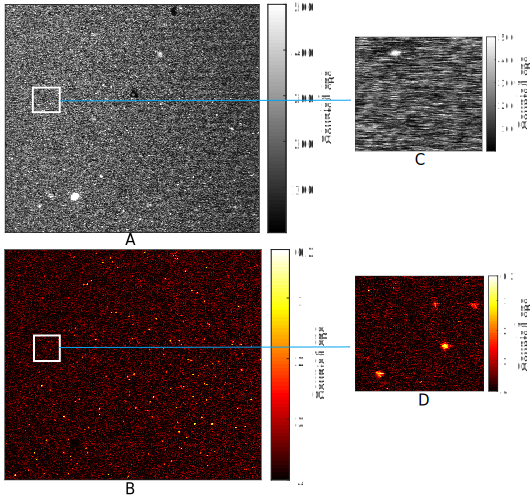
\includegraphics[width=0.8\textwidth]{xy_with_zoom.png}
  \makeatletter
  \renewcommand{\fnum@figure}{\figurename~S\thefigure}
  \makeatother{}
  \caption{ Intensity image (A) and lifetime image (C) of a $80~\um\times80~\um$ area of a glass substrate with spin-coated gold nanorods and covered with a supported lipid bilayer. The bilayer is labeled by incubation with 100~\nM~ATTO 647N. Intensity image (B) and lifetime image (D) of a zoomed-in area of the original imag}
  \label{SIfig:xy-scan}
\end{figure}

A large area of the bilayer labeled with ATTO 647N can be seen in Figure S\ref{SIfig:xy-scan}A. The intensity is almost uniform across the whole area except for some bright and dark spots. The bright spots are
probably un-ruptured vesicles and the dark spots indicate holes in the bilayer. Measurements
described in the text have been conducted far away from these holes. The bright spots in the
lifetime image (Fig.S\ref{SIfig:xy-scan}C) indicate the nanorods. Most of the bright spots in the intensity image don't correlate with the bright spots in the lifetime image. This is the reason we rely on the
lifetime image to locate the gold nanorods.\\

\newpage
\section{Zooming in on intensity bursts}
\begin{figure}[ht]
  \centering
  \includegraphics[width=0.8\textwidth]{zoomed_traces.png}
  \makeatletter
  \renewcommand{\fnum@figure}{\figurename~S\thefigure}
  \makeatother{}
  \caption{Zoomed-in time traces of the enhanced bursts (A-E) observed for ATTO 647N in the presence of gold nanorod showing that the enhanced signal nearly always is embedded in the far field signal; (F) Time trace of ATTO 647N in the bilayer in the absence of gold nanorod. The full time traces were shown in Figure 1.}
  \label{SIfig:zoomed-trace}
\end{figure}
Figure S\ref{SIfig:zoomed-trace}A-E shows different enhanced bursts observed when ATTO 647N molecules diffuse around a gold nanorod. The distinction is made on the basis of intensity. Intensity levels above 100 kcps represent enhanced signals and have been marked by a dotted box. In all the bursts shown it can be seen that the near-field signal is observed only in the presence of the far-field signal. A molecule travels some distance in the far field before it reaches the near field. In absence of gold nanorod (Fig. S\ref{SIfig:zoomed-trace}F), we only see the far-field signal and no short bursts, as expected.\\
\newpage
\section{Fitting of FCS curves}
As only probe molecules in the bilayer contribute to the signal, the FCS curves without nanorod
were fitted with a two-dimensional Gaussian model:
\begin{equation}
	G_{FF}(\tau)-1 = \frac{1}{N_{FF}}\Bigg(1+\frac{\tau}{\tau_{FF}}\Bigg)
	\label{eq:2Dgauss}
\end{equation}
where $_{FF}$ represents the average number of molecules in the focal spot and $\tau_{FF}$ is the diffusion time in the focal spot. The amplitude of the autocorrelation, $G(0)-1$ directly gives the average number of fluorescent species in the detection volume, $N=[G(0)-1]^{-1}$. At incubation with a solution of 100~\nM ATTO 647N in buffer, the average number of molecules in the bilayer appeared to be 35. Background corrections were negligible.\\
The gold nanorod enhances fluorescence and the enhanced signal in the near-field of the gold nanorod was observed only in the presence of the far field (diffraction limited area) signal.(Vide supra).\\
\begin{figure}[ht]
  \centering
  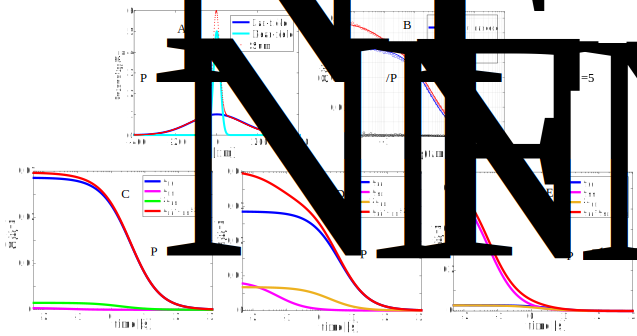
\includegraphics[width=\textwidth]{calc_enhc_corr.png}
  \makeatletter
  \renewcommand{\fnum@figure}{\figurename~S\thefigure}
  \makeatother{}
  \caption{(A) crosscut (red dots) through an intensity profile consisting of the sum of two Gaussians: Far-field Gaussian (blue, waist=265 nm; peak height: $P_{FF}=1$) and near-field Gaussian (magenta, $waist=31~\nm$; peak height: $P_{NF}=5$). (B) Experimental autocorrelations of fluorescence intensity traces at 100~\nM ATTO 647N in presence of the rod (red circles), in the absence of the rod (blue circles), and of the gold luminescence only (black circles, in absence of ATTO 647N). (C-E) Calculated autocorrelation for the entire intensity profile (red) and its constituents: the autocorrelation of far-field focus AFF (blue), the near-field $A_{NN}$ (magenta) and the sum of identical cross-terms $2A_{FN}$ (green) with different peak heights $P_{FN}/P_{FF}=1$(C), $P_{FN}/P_{FF}=5$(D) and $P_{FN}/P_{FF}=90$(E). The calculated correlations fit best the experimental correlations for a peak height ratio of 5. This value is very close to the maximum factor of 4 enhancement obtained from direct comparison of burst intensities (main text).}
  \label{SIfig:calc_enhc_corr}
\end{figure}
The theoretical model of the correlation function was compared to experimental correlation functions. In the model of Langguth and Koenderink\cite{langguth2016exact}, the molecule detection function is considered as the superposition of two coinciding 2D Gaussians. We take a beam waist of 265~\nm for the far field and 31~\nm for the near-field. The total correlations were calculated as:
\begin{equation}
	G(\tau)-1 = \frac{1}{<C>S_{MDF}^2}[\sum_{n}A_{nn}(\tau) + \sum_{n\neq m}A_{nm}(\tau)],
	\label{eq:far-near-gauss}
\end{equation}
with n, m = F (far-field), or N (near-field),
\begin{equation}
	A_{n,m}(\tau)=S_nS_m\Bigg[\frac{2}{\pi\Big([\omega_n]^2 + [\omega_m^D(\tau)]^2 \Big)}\Bigg] ,
	\label{eq:area-gauss}
\end{equation}
$\omega_m^D(\tau)=\sqrt{\omega_m^2 + *D\tau}$, $S_n=P_n\times A_n$ and $S_{MDF}^2=\Big[\sum_{n}S_n\Big]^2$,\\
where $P_n$ indicates the peak intensity and $A_n$ the area of the Gaussian distribution. Figure S\ref{SIfig:calc_enhc_corr}C-D shows calculated correlations for different peak intensity ratio ($P_F/P_N$). The red curved indicates the total correlation function and the other curves represent individual correlations (blue, green and magenta) that contribute to the total correlation. Here we would like to emphasize that the contribution of the cross terms (AFN) between far-field and near-field is not negligible, especially at low peak intensity ratios.

\section{Lifetime-based selection}
\begin{figure}[ht]
  \centering
  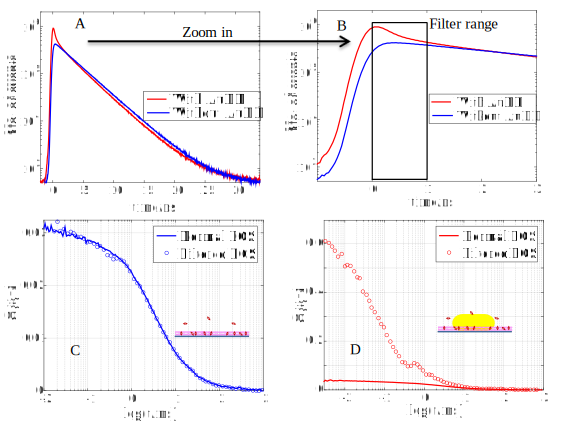
\includegraphics[width=0.8\textwidth]{lifetime_filtering.png}
  \makeatletter
  \renewcommand{\fnum@figure}{\figurename~S\thefigure}
  \makeatother{}
  \caption{Filtering signal. (A) Fluorescence decay of 100~\nM of ATTO 647N in the presence (blue) and absence (red) of a gold nanorod. (B) Zoomed-in part of the decay in Fig.S\ref{SIfig:lifetime-filtering}A at shorter time scales. The dotted box indicates the range of arrival time of fluorescence counts considered for filtering the enhanced signal. The autocorrelation of normal and filtered time traces in absence (C) and presence (D) of nanorods. Notice the invariance of the correlation in the absence of nanorods and the significant improvement in the correlation contrast in presence of the nanorod.}
  \label{SIfig:lifetime-filtering}
\end{figure}
Correlation for shorter lifetime photons (enhanced signal) was obtained using only the photons arriving within 1 ns after the excitation pulse. The blue decay in Figure S\ref{SIfig:lifetime-filtering}A represents the fluorescence decay of ATTO647N in the absence of gold nanorods and the red one in the presence of the gold nanorod. It can be clearly seen that the lifetime histogram in presence of the nanorod exhibits a multicomponent decay. All the photons falling in the dotted box in Figure S\ref{SIfig:lifetime-filtering}B were selected for correlation. While the FCS curve in the absence of the nanorod remained unchanged as can be seen in Figure S\ref{SIfig:lifetime-filtering}C, the FCS contrast within the presence of gold nanorods showed a significant improvement. This is because of the selective consideration of the enhanced signal in the near field and suppression of background coming from far field.

\section{Effect of cut-off range}
\begin{figure}[ht]
  \centering
  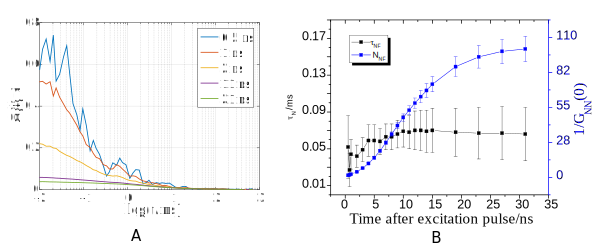
\includegraphics[width=0.9\textwidth]{cutoff_effect.png}
  \makeatletter
  \renewcommand{\fnum@figure}{\figurename~S\thefigure}
  \makeatother{}
  \caption{Effect of cut-off range. (A) Autocorrelation of time trace of ATTO 647N after lifetime filtering. The corresponding times after the excitation pulse are shown in the legend. Notice the significant increase in the noisiness between filtering times 1~\ns (red) and 0.5~\ns (blue). (B) Effect of the selection time window on the near-field correlation parameters. The near-field diffusion time is shown in black indicating minimal changes of time with selection range, whereas the number of molecules in the near field, shown in blue, undergoes a significant reduction.}
  \label{SIfig:cutoff-effect}
\end{figure}

\section{Fluorescence enhancement in 3D diffusion}
Fluorescence enhancement experiments were performed with 10\nM ATTO 647N in 70\% sucrose solution and gold nanorods on glass substrate. We observed an average intensity of 50 kcps observed for five molecules in the diffraction-limited volume in the absence of gold nanorods. The intensity from a single molecule was 10 kcps. In presence of gold nanorods, bursts with a maximum of 1200 kcps were observed corresponding with an enhancement factor of 110. (Figure S\ref{SIfig:cutoff-effect})\\
\begin{figure}[ht]
  \centering
  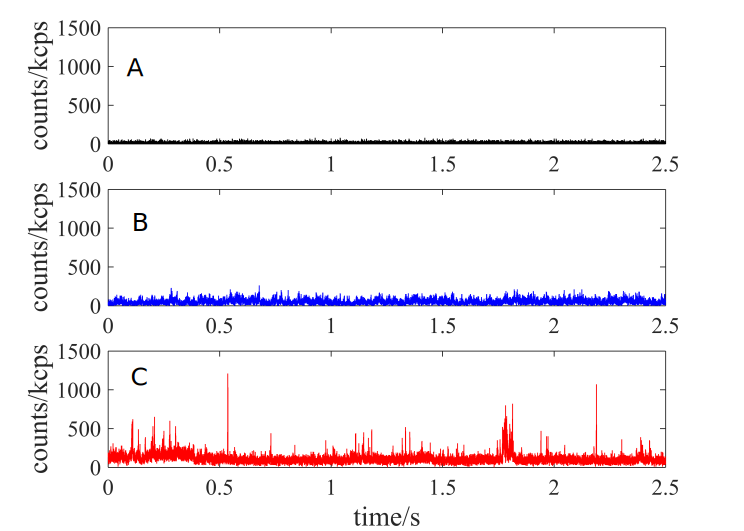
\includegraphics[width=\textwidth]{3D_enhc.png}
  \makeatletter
  \renewcommand{\fnum@figure}{\figurename~S\thefigure}
  \makeatother{}
  \caption{Time traces with a binning time of 100~\us of (A) Gold nanorod in sucrose with a constant intensity of 20 kcps; (B) ATTO647N without gold nanorod in sucrose with average intensity of 51 kcps for 5 molecules on average, as obtained from the autocorrelation function. This translates into a brightness of 10 kcps per molecule; (C) ATTO 647N with gold nanorod in sucrose with a maximum intensity of 1200 kcps. Hence the fluorescence of ATTO 647N was enhanced by a factor of 110 by the gold nanorod.}
  \label{SIfig:3D-enhc}
\end{figure}
The enhancement factor of 110 is far bigger than the factor of 4 observed in the case of the lipid bilayer. The lifetime remained the same both in the bilayer and in the sucrose solution indicating no change in the quantum yield. The difference in the enhancement factor can be explained by the accessibility of the hot spot for the diffusing molecules. The nanorod used in the experiment is 50~\nm thick. In case of a bilayer, we suppose that the molecules are confined at the bottom to a layer of 5~\nm thick. Hence the diffusing molecules are not able to explore the most intense region of the hot spot, resulting in a weaker enhancement. In the case of sucrose, however, the dye molecules diffuse through the whole space around the nanorod and occasionally reach the intense hot spot region resulting in a larger maximum fluorescence enhancements. This observation confirms the assumption that the bilayer does not cover the tips of the rod.\\
\newpage
\section{Partitioning of the dye between surface and solution}
\begin{figure}[ht]
  \centering
  \includegraphics[width=\textwidth]{surf_soln.png}
  \makeatletter
  \renewcommand{\fnum@figure}{\figurename~S\thefigure}
  \makeatother{}
  \caption{A) Time traces with a binning time of 1~\ms of ATTO 647N on surface (blue) with an average intensity of 235 kcps and in solution (green) with an average intensity of 60 kcps. (B) Autocorrelation of time traces of ATTO647N on surface (blue) and solution (green). Notice the absence of correlation component corresponding to the solution in the blue curve. The high background from the surface suppresses the correlation contrast of the dye in solution. The similar magnitude of the autocorrelation contrasts indicates that the number of molecules on the surface is almost the same as the number of molecules in the three-dimensional detection volume in solution. As the dye has a certain partition coefficient between the surface of the bilayer and the solution, the dye content on the surface can be controlled simply by changing the dye concentration in the solution.}
  \label{SIfig:surf-soln}
\end{figure}

\pagebreak
\bibliographystyle{ieeetr} % For a list of bibliography styles, see https://www.sharelatex.com/learn/Bibtex_bibliography_styles
\bibliography{efcs}
\end{document}